% Research theme figure: Flow Through Porous and Subsurface Media
% (pore scale -> volume averaging (REV) -> reservoir scale). Same canvas, fonts and
% palette as the other research figures; greyscale on the site, colour on hover.
% Build (from this folder):
%   latex porous.tex
%   dvisvgm --no-fonts --bbox=papersize -o ../porous.svg porous.dvi
\def\pgfsysdriver{pgfsys-dvisvgm.def}
\documentclass[tikz,border=0pt]{standalone}
\usetikzlibrary{arrows.meta}
\renewcommand{\familydefault}{\sfdefault}

% --- palette (shared with the other research figures) ------------------------
\definecolor{ink}{HTML}{1A1A1A}
\definecolor{frame}{HTML}{4D4D4D}
\definecolor{steel}{HTML}{245A94}
\definecolor{sky}{HTML}{6E9FD2}
\definecolor{mist}{HTML}{D3E3F3}
\definecolor{amber}{HTML}{C8702A}
\definecolor{sand}{HTML}{F0CFA8}

\begin{document}
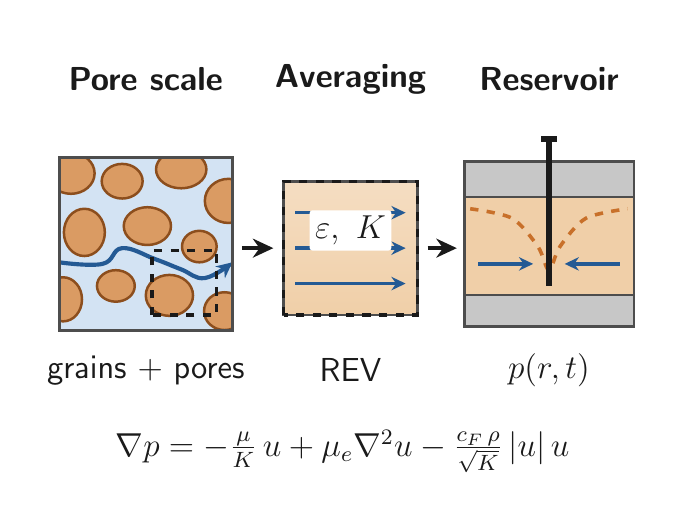
\begin{tikzpicture}[
    line width=1.6pt, >={Stealth[length=2.6mm,width=2.4mm]},
    small arrow/.style={-{Stealth[length=1.8mm,width=1.7mm]}, line width=1.2pt},
    color=ink,
    title/.style={font=\large\bfseries, text=ink},
    lab/.style={font=\large, text=ink},
    grain/.style={fill=amber!55!sand, draw=amber!70!black, line width=0.9pt}]
  % fixed 8 cm x 6 cm canvas
  \path[use as bounding box] (0,0) rectangle (8,6);

  % ================= 1) pore scale: grains, pore fluid, streamline =================
  \node[title] at (1.50,5.35) {Pore scale};
  \begin{scope}
    \clip (0.40,2.15) rectangle (2.60,4.35);
    \fill[mist] (0.40,2.15) rectangle (2.60,4.35);
    % grains (solid matrix)
    \foreach \x/\y/\a/\b in {0.55/4.15/0.30/0.26, 1.20/4.05/0.26/0.22, 1.95/4.20/0.32/0.24, 2.55/3.80/0.30/0.28,
                             0.72/3.40/0.26/0.30, 1.52/3.48/0.30/0.24, 2.18/3.22/0.22/0.20,
                             0.45/2.55/0.24/0.28, 1.12/2.72/0.24/0.20, 1.80/2.60/0.30/0.26, 2.50/2.40/0.26/0.24}
      \draw[grain] (\x,\y) ellipse ({\a} and {\b});
    % streamline threading the pore space
    \draw[steel, line width=1.5pt, -{Stealth[length=2.0mm,width=1.9mm]}]
      plot[smooth, tension=0.7] coordinates
        {(0.40,3.02) (0.95,3.00) (1.20,3.20) (1.62,3.06) (1.95,2.93) (2.25,2.82) (2.60,3.02)};
  \end{scope}
  \draw[frame, line width=1.0pt] (0.40,2.15) rectangle (2.60,4.35);
  % REV (averaging window)
  \draw[ink, line width=1.2pt, dashed] (1.58,2.35) rectangle (2.40,3.17);
  \node[lab] at (1.50,1.65) {grains + pores};

  % ================= 2) volume averaging -> porous continuum =================
  \node[title] at (4.10,5.35) {Averaging};
  \shade[top color=sand!70!white, bottom color=sand, draw=frame, line width=1.0pt]
    (3.25,2.35) rectangle (4.95,4.05);
  \draw[ink, line width=1.2pt, dashed] (3.25,2.35) rectangle (4.95,4.05);
  \foreach \y in {2.75,3.20,3.65}
    \draw[steel, small arrow] (3.40,\y) -- (4.80,\y);
  \node[fill=white, inner sep=2pt, rounded corners=1pt, font=\large, text=ink] at (4.10,3.425) {$\varepsilon,\ K$};
  \node[lab] at (4.10,1.65) {REV};

  % ================= 3) reservoir scale: layer, well, drawdown =================
  \node[title] at (6.62,5.35) {Reservoir};
  % cap rock, reservoir, base rock
  \fill[black!22] (5.55,3.85) rectangle (7.70,4.30);
  \fill[sand] (5.55,2.60) rectangle (7.70,3.85);
  \fill[black!22] (5.55,2.20) rectangle (7.70,2.60);
  \draw[frame, line width=1.0pt] (5.55,2.20) rectangle (7.70,4.30);
  \draw[frame, line width=0.8pt] (5.55,3.85) -- (7.70,3.85) (5.55,2.60) -- (7.70,2.60);
  % pressure drawdown cone toward the well
  \draw[amber, line width=1.3pt, dashed]
    plot[smooth, tension=0.5] coordinates {(5.62,3.70) (6.15,3.58) (6.48,3.22) (6.62,2.92) (6.76,3.22) (7.09,3.58) (7.62,3.70)};
  % radial inflow to the well
  \draw[steel, small arrow] (5.72,3.00) -- (6.42,3.00);
  \draw[steel, small arrow] (7.52,3.00) -- (6.82,3.00);
  % well
  \draw[ink, line width=2.2pt] (6.62,4.55) -- (6.62,2.72);
  \fill[ink] (6.52,4.55) rectangle (6.72,4.62);
  \node[lab] at (6.62,1.65) {$p(r,t)$};

  % ================= arrows between panels =================
  \draw[->] (2.72,3.20) -- (3.12,3.20);
  \draw[->] (5.08,3.20) -- (5.45,3.20);

  % ================= Darcy-Brinkman-Forchheimer momentum balance =================
  \node[font=\large, text=ink] at (4.00,0.62)
    {$\nabla p = -\frac{\mu}{K}\,u + \mu_e\nabla^2 u - \frac{c_F\,\rho}{\sqrt{K}}\,|u|\,u$};
\end{tikzpicture}
\end{document}
